\documentclass[12pt,avenir,a4paper,final]{iopart}
\usepackage{iopams}  
\linespread{1.5}
\usepackage{graphicx}
\usepackage[tmargin=4cm, lmargin=3cm, rmargin=3cm]{geometry}
\usepackage[breaklinks=true,colorlinks=true,linkcolor=blue,urlcolor=blue,citecolor=blue]{hyperref}
\usepackage{mwe}
\usepackage{subfig}
%\usepackage{caption,subcaption}
\newenvironment{nstabbing}
  {\setlength{\topsep}{0pt}%
   \setlength{\partopsep}{0pt}%
   \tabbing}
  {\endtabbing}
%\usepackage{subcaption}
\captionsetup[figure]{labelfont=bf,labelsep=period}
\captionsetup[subfigure]{labelfont=bf,textfont=normalfont}
\captionsetup[subfigure]{labelformat=simple}
\renewcommand\thesubfigure{(\alph{subfigure})}
\makeatletter
\newcommand*{\rom}[1]{\expandafter\@slowromancap\romannumeral #1@}
\makeatother
\setlength{\belowcaptionskip}{-3pt}
\makeatletter
\def\footnoterule{\kern-3\p@
  \hrule \@width 2in \kern 2.6\p@} 
\makeatother
\begin{document}
\maketitle
 
\title[P2P Report]{P2P Report}
\author{Husni Almoubayyed}
\address{School of Physics and Astronomy, University of Glasgow}
\eads{\mailto{2061022a@student.glasgow.ac.uk}}

\section{Introduction}
\indent \par{}I enrolled in the peer teaching course with no previous insight or experience in teaching. I was hoping to gain a new range of skills, contribute to the education of students in lower years, and become more prepared to potential future positions. Overall, it exceeded my expectations, and I plan to teach as part of (but not completely central to) my academic research career. It was beneficial and satisfying in several other aspects, such as strengthening my general physics knowledge, and honing my rhetorical skills. 

\section{Experiences as a Peer Tutor}
\label{1}
\indent \par{} About half the time, I was asked the \emph{what's the final answer?} sort of questions, and in most of the cases, having a tutor answer that question can be only as helpful as having a sheet of paper answer it. However, the other half of the time was the one more interesting. I felt my teaching skills increasing with every tutorial, and I noticed myself getting much better at things such as using hints to lead the students towards the correct answer, rather than jumping directly to it, and explaining the underlying physical concepts within the tutorial problems. At some points, I found myself telling the students about how their courses will evolve in the following years and what to expect, (sometimes promising them that \emph{they will know where ``this comes from" in a few years' time.} see e.g. journal entry 9), which I was told was quite helpful to them. 

\indent \par{}Although the number of tutors was arguably large and more tutors than necessary were present at most tutorials, I think that it was still helpful, because it allowed us to discuss both issues related to teaching and to earlier years' content. At some points this auspiciously led to giving the students answers from different perspectives and approaches, letting them decide which approach works best for them.

\indent \par{}  Some other observations that I made were that the student attendance declined steadily throughout the year, perhaps making all the tutorials assessed would improve attendance. The amount of questions students ask also declined, hopefully because they study more as the year progresses, and not because they are not finding the tutorials helpful enough to ask questions.

\indent \par{} I also found that the students seemed convinced of what the tutors tell them more as the year advanced, probably because of the combination that trust was built up between the tutors and tutees, and because the tutors' rhetorical skills improved a lot throughout the course, which I believe plays a large role in teaching.

\section{Teaching Philosophy}
\label{2}
\indent \par{} The peer teaching course has definitely helped shape my teaching philosophy and techniques. While everything was kept to quite a basic level, it was sufficient as a first exposure to teaching, while also encouraging me to start thinking about how to form a unique teaching philosophy. My techniques in this course included things such as asking the students whether they have questions every now and then rather than always waiting for questions (which I found that most of the times they do have questions but are too shy to ask), and rechecking with the students some time after helping them to see if they were able to solve the rest of the questions successfully (I found that most of the times the students get stuck on the same question, one or two steps afterwards). 

\indent \par{} Experiencing peer tutoring also influenced my future teaching philosophy, and gave me some ideas about what I would like to do in classes I would potentially teach in the future, for example, I think discussions amongst students are lacking in the current methods. This can be overcome by encouraging students to participate in classes-specific online forums -- perhaps on Moodle or similar services.

\section{Further Implementations of P2P Teaching}
\indent \par{} I asked a moderate sample of students to give feedback about the peer tutorials, and most agreed that peer teaching is not as helpful as it can be. I agree that it has a lot of potential in the sense that it can be implemented beyond just helping with the tutorials. The drop in tutorials were a unique type of tutorials, which I think were most helpful to the students. I think this can be taken as far as to assign supervision groups to peer tutors, where students email the tutors their questions beforehand and then attend the supervisions, in a similar manner to upper-year supervisions. Peer teachers can furthermore set office hours (where e.g. a conference room can be used). I expect that peer tutors would also be able to help with labs, practical work, and in co-supervising research, and helping with academic writing.

\section{P2P Observation Feedback Response}
\indent \par{}
In the observed tutorial, the observer found that I go too much in-depth when explaining the underlying physics and go beyond the students' level of knowledge. It can indeed be very tricky sometimes to explain the physical concepts without going onto complicated ideas and it is definitely an acquired but important skill to always talk appropriately to different audiences with specific level of knowledge on a certain subject, and it is one skill that I aim to acquire. We also take too many things for granted that students in lower years find challenging. On the other hand, I think it is essential to spend some time explaining the underlying physics, because classes can most of the times be too mathematical, and students do not get enough chances to think about the physical background. 

\indent \par{} The observer also found that I often let the students work on things they do not know and do not have a big chance of working though for too long and let them struggle before giving assistance. While I agree that letting students' minds diverge too much before leading them to the right track is not always the best approach, I still believe that the questions that the students struggle with most, and the concepts that they spend a lot of time thinking about, are the ones that they will remember most for the longest time. 

\indent \par{} I am glad that the observer found that I was successful with giving hints and clues to the answers, and leading the students to the answers well, without jumping to them directly myself, as it has taken me most of the first semester to achieve this well. I believe the rest of the observer's comments reflect consistently on what I mentioned in sections~\ref{1} and~\ref{2} above, particularly, about having discussions with other tutors about the (sometimes ambiguous) questions and content of the tutorials.
\section{Conclusion}
\indent \par{} My experiences grew vastly throughout the course of the P2P module, which was also my first exposure to teaching in general. It has influenced my perspective on teaching, and encouraged me to participate in  teaching opportunities that I get in my future career in academia. Throughout the year I answered the students' questions in physics tutorials, but I was also able to relate to them, at times answering their questions and expectations about their following years. In addition to leading the students to answering the tutorial questions, I was able to explain the physical concepts behind the more mathematically-minded lecture courses that they study. I also participated in discussing the content, and different approaches to the answers with fellow tutors. In addition, I made a few observations that changed throughout the years, such as the declining number of students attending the tutorials, and suggested possible solutions, for example, making the tutorials assessed. The peer teaching module has furthermore influenced me to think thoroughly about my teaching philosophy and about forming a unique approach to teaching. What's more, it  encouraged me to think about the potential of peer teaching and its possible applications in supervising tutees, helping them with laboratory and practical work, and giving them advice on academic writing. There are still issues that I need to work on emphasised in the feedback I received from the observing session, mainly in terms of my ability to explain physical concepts clearly to an audience with quite a specific level of knowledge in physics, and in finding the appropriate balance between giving assistance and letting the students wander off to explore different approaches in answering the questions. Overall, it was an enjoyable experience that left me both prepared and excited to become a teaching assistant in the following years as a postgraduate student. 
\indent \par{} 
%\footnotesize {word-count = 1399 by \href{http://app.uio.no/ifi/texcount/}{\TeX count}}
\clearpage
\section*{Appendix: Observing Report}
\begin{figure}[htbp]
\begin{center}
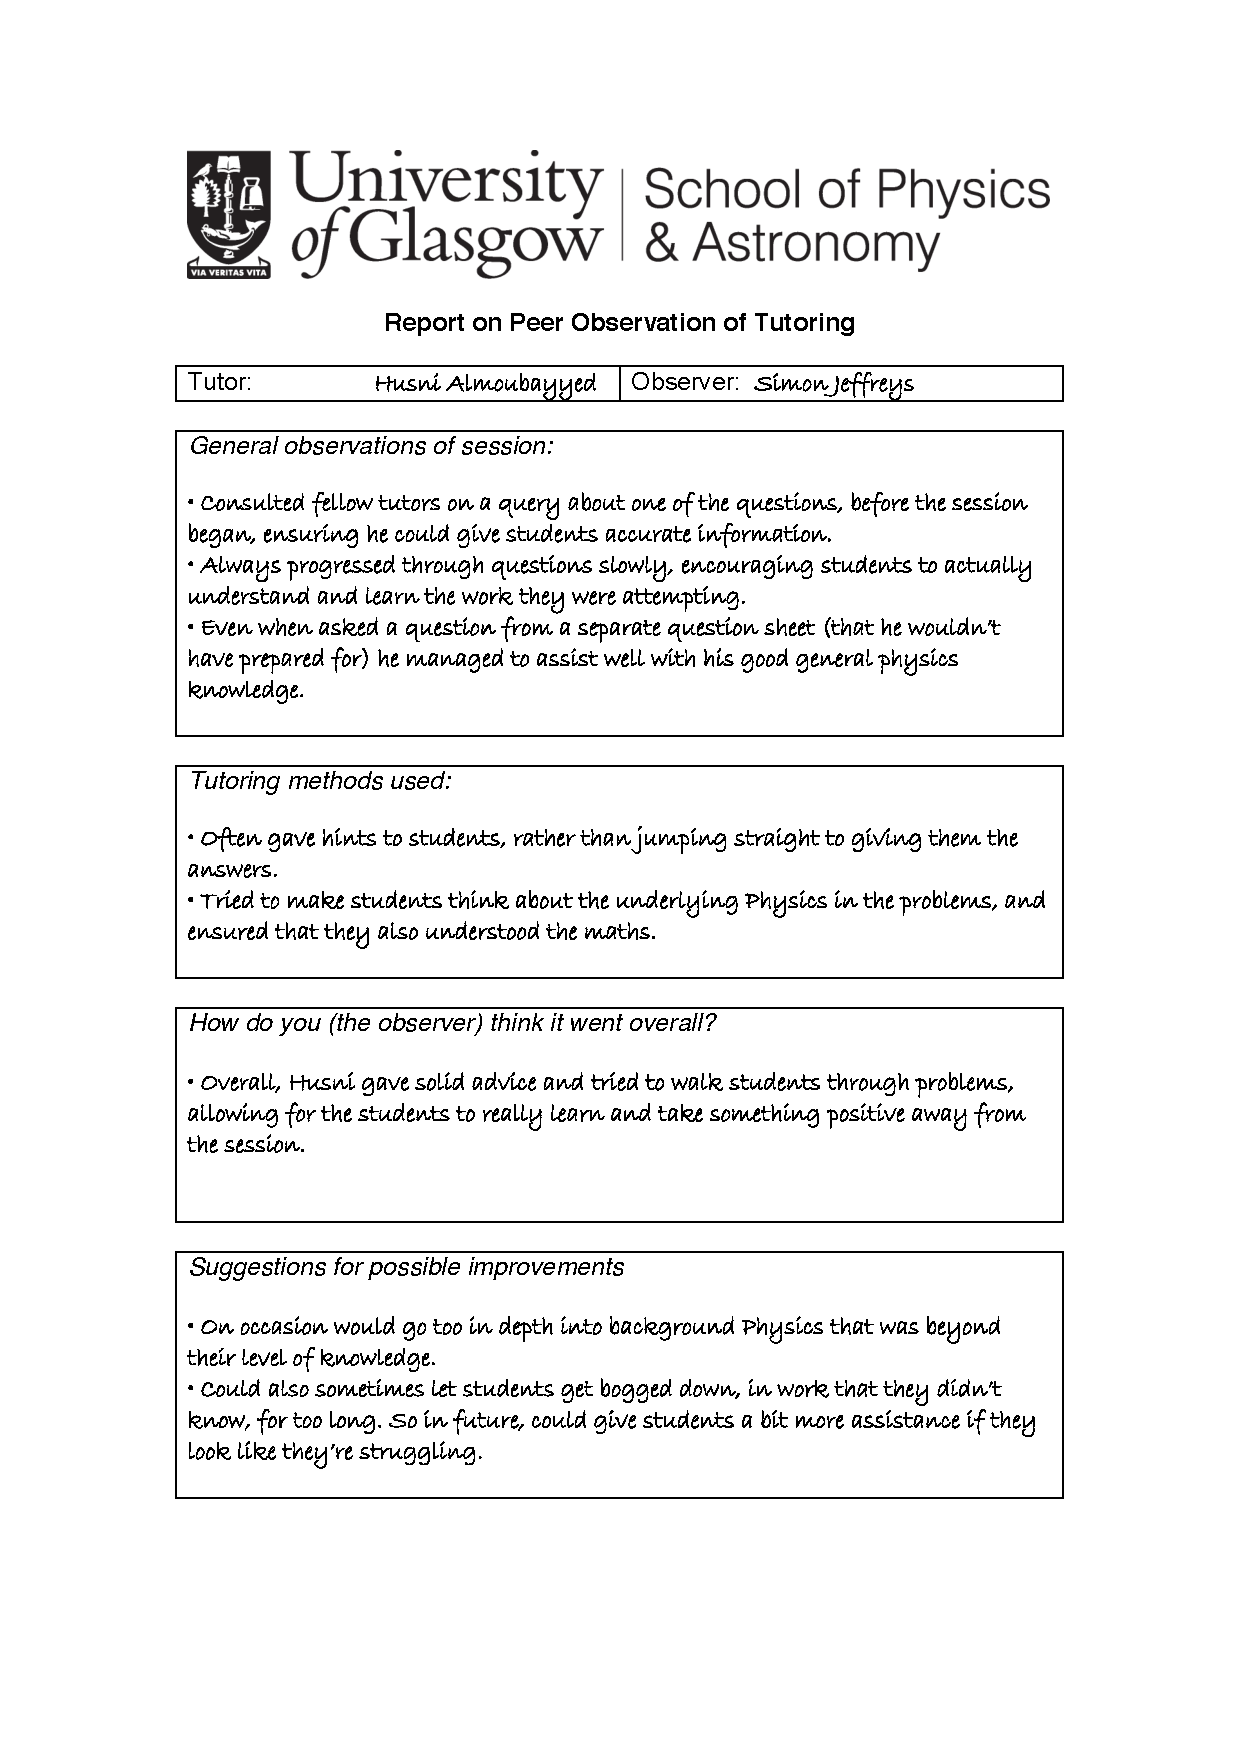
\includegraphics[width=0.9\textwidth]{feedback}
\end{center}
\end{figure}

\end{document}